\appendix

\section{Runtime heterogeneity and the mechanism of cost-aware acquisition}

\subsection{Runtime scale and recoverability}
\label{app:predicted-runtime}

Algorithm identity provides a strong first-order cost signal (Figure~\ref{fig:runtime_dist}), but a single average does not describe the observed within-engine tails. Uni-Mol and the two DiffDock variants are consistently costly, whereas Smina and SurfDock are usually cheap. AutoDock Vina is a consequential exception: its median is below those of Uni-Mol and the DiffDock variants, but its upper tail spans orders of magnitude. Cost-aware acquisition therefore encounters both between-algorithm scale differences and within-algorithm tail risk. AutoDock Vina has a median runtime of $12$\,s but a mean of $48.4$\,s and accounts for $42.7$ of the $123.2$ hours required by the full matrix.

\begin{figure}[!htb]
\centering
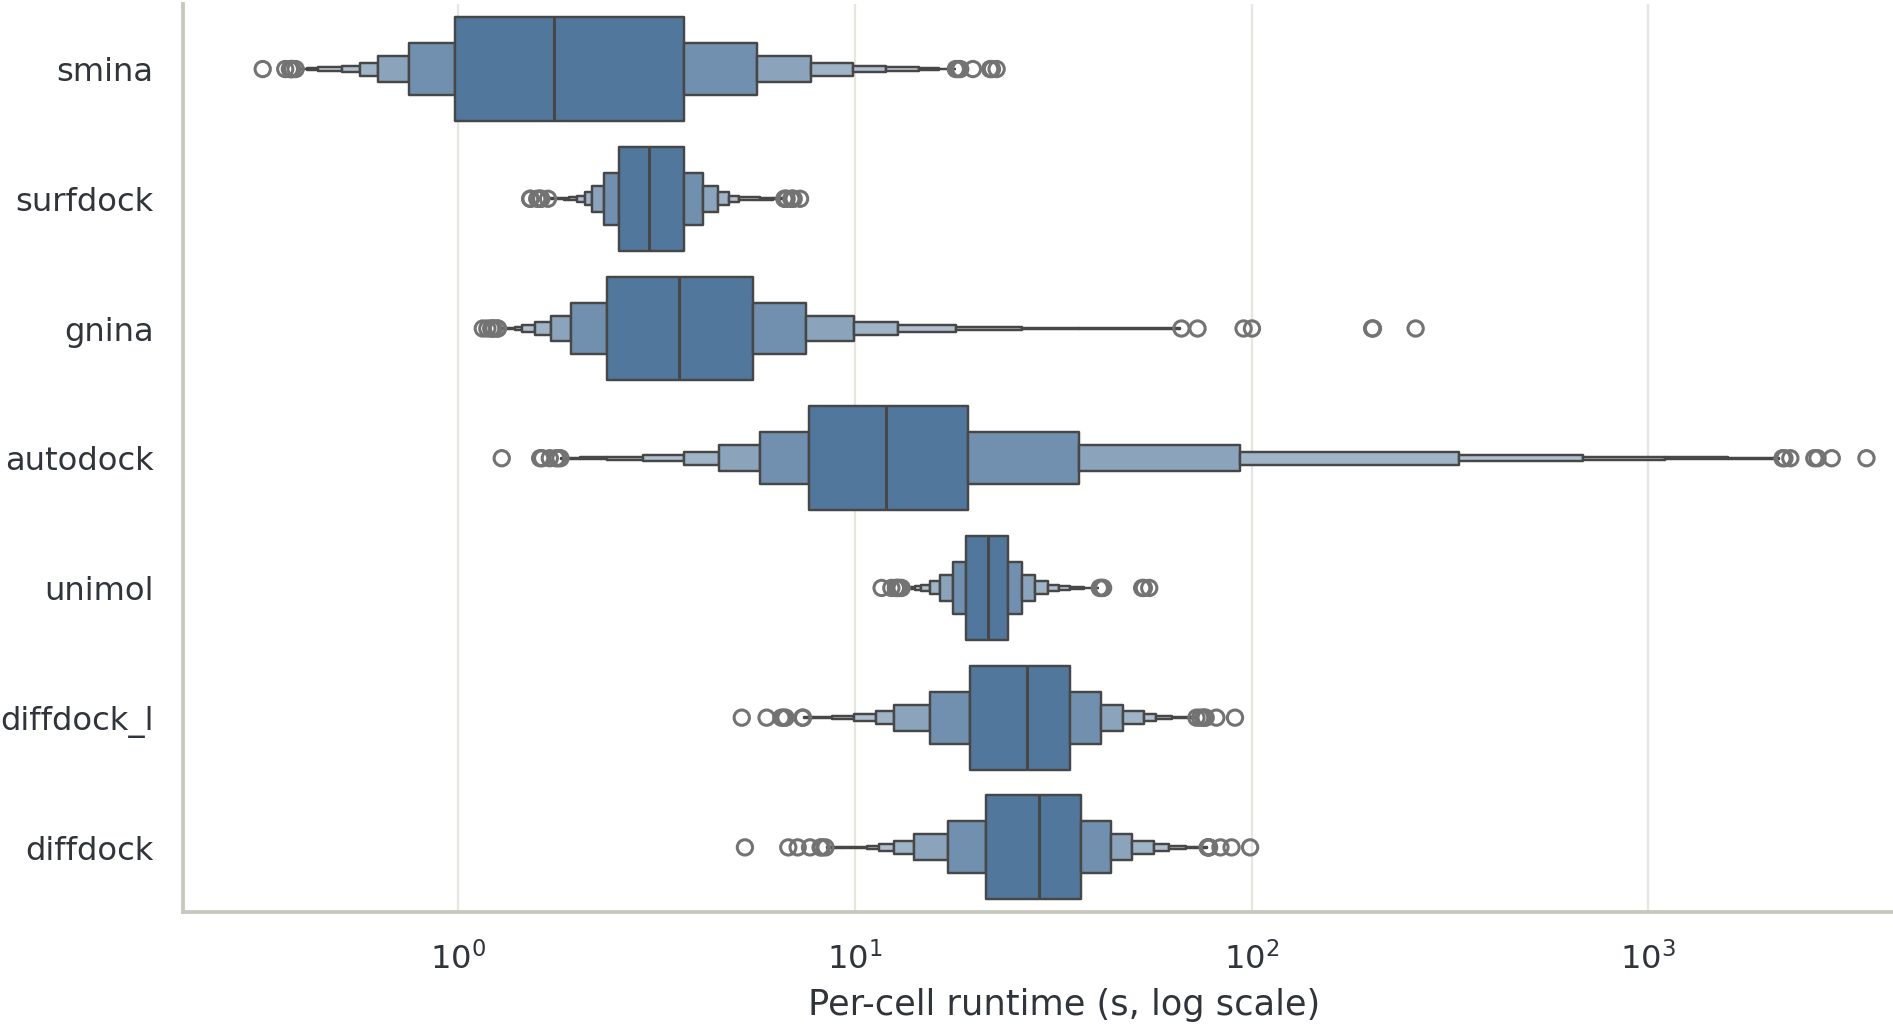
\includegraphics[width=\linewidth]{figures/runtime_distribution-REV.png}
\caption{Per-cell runtime distributions across 3,179 MOAD-curated complexes.}
\label{fig:runtime_dist}
\end{figure}

\begin{figure}[!htb]
\centering
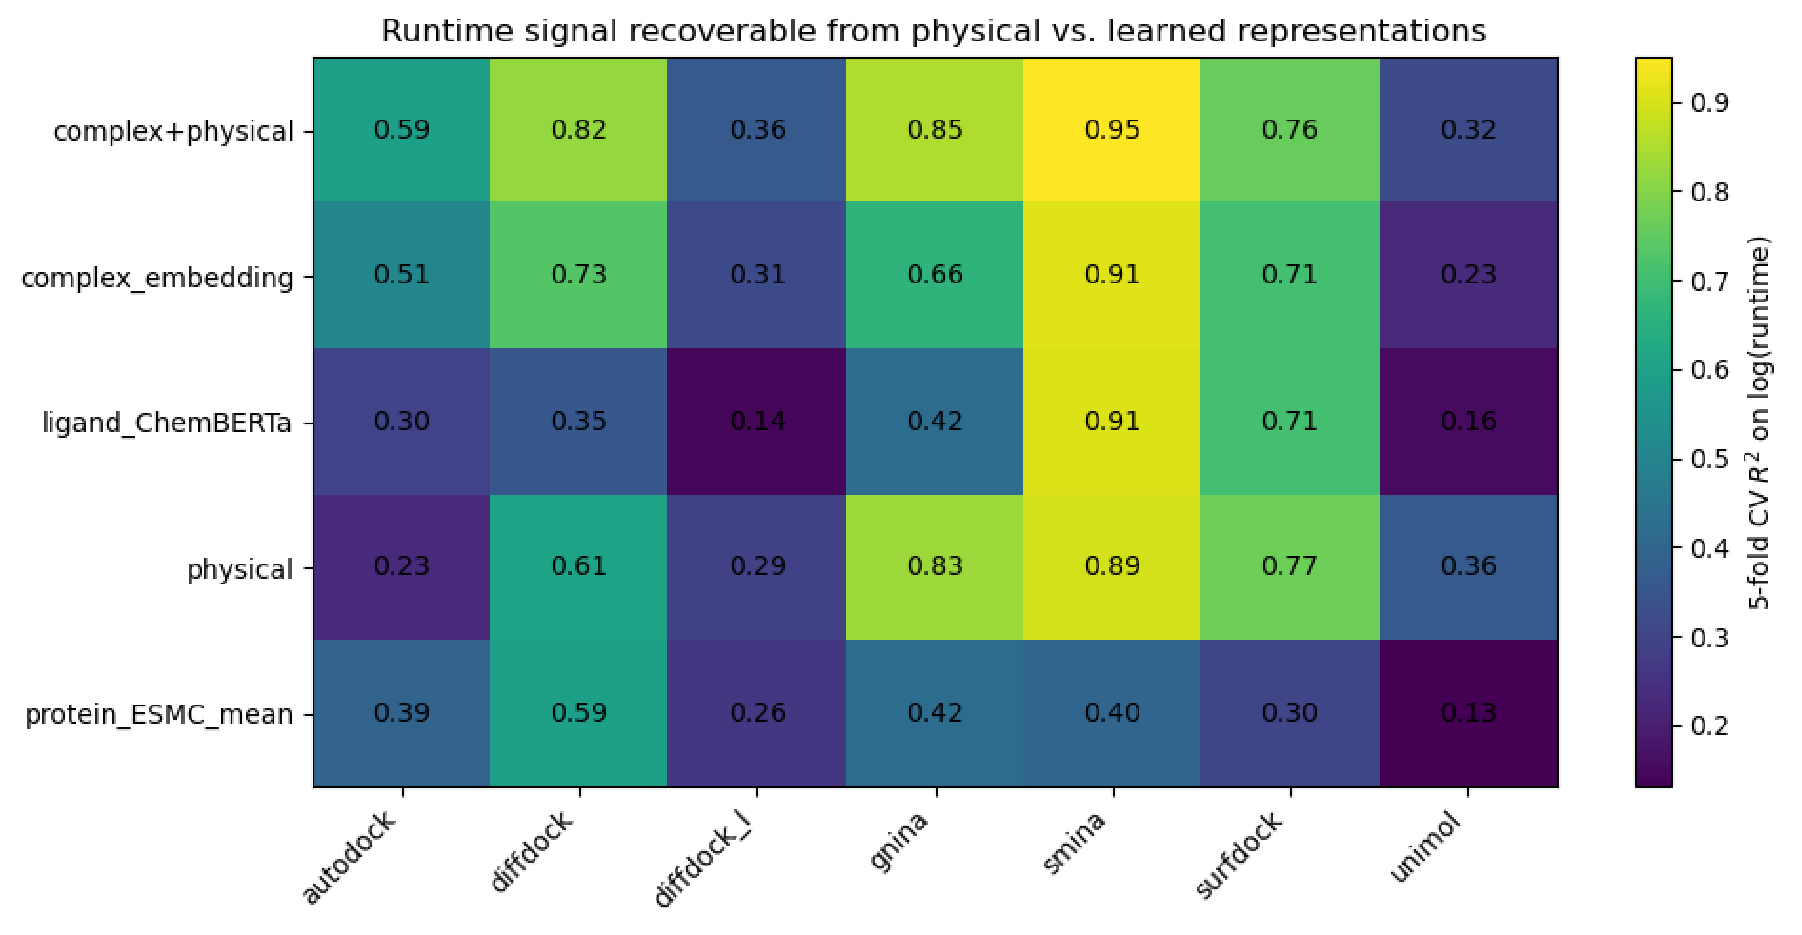
\includegraphics[width=\linewidth]{figures/cost_predictability.pdf}
\caption{Mean five-fold cross-validation $R^2$ from engine-specific ridge probes on log runtime.}
\label{fig:cost_predictability}
\end{figure}

The ridge probes in Figure~\ref{fig:cost_predictability} show that runtime is linearly predictable from the available features for some engines under this diagnostic protocol. The combined complex representation and physical descriptors explain log runtime well for Smina, GNINA, DiffDock, and SurfDock, but only moderately for AutoDock Vina and weakly for DiffDock-L and Uni-Mol. Adding representations is not uniformly beneficial. A low probe $R^2$ does not establish that nonlinear prediction is impossible. Conversely, probe performance does not validate the calibration of the acquisition-time MLP trained on selectively observed runtimes.

\begin{figure}[!htb]
\centering
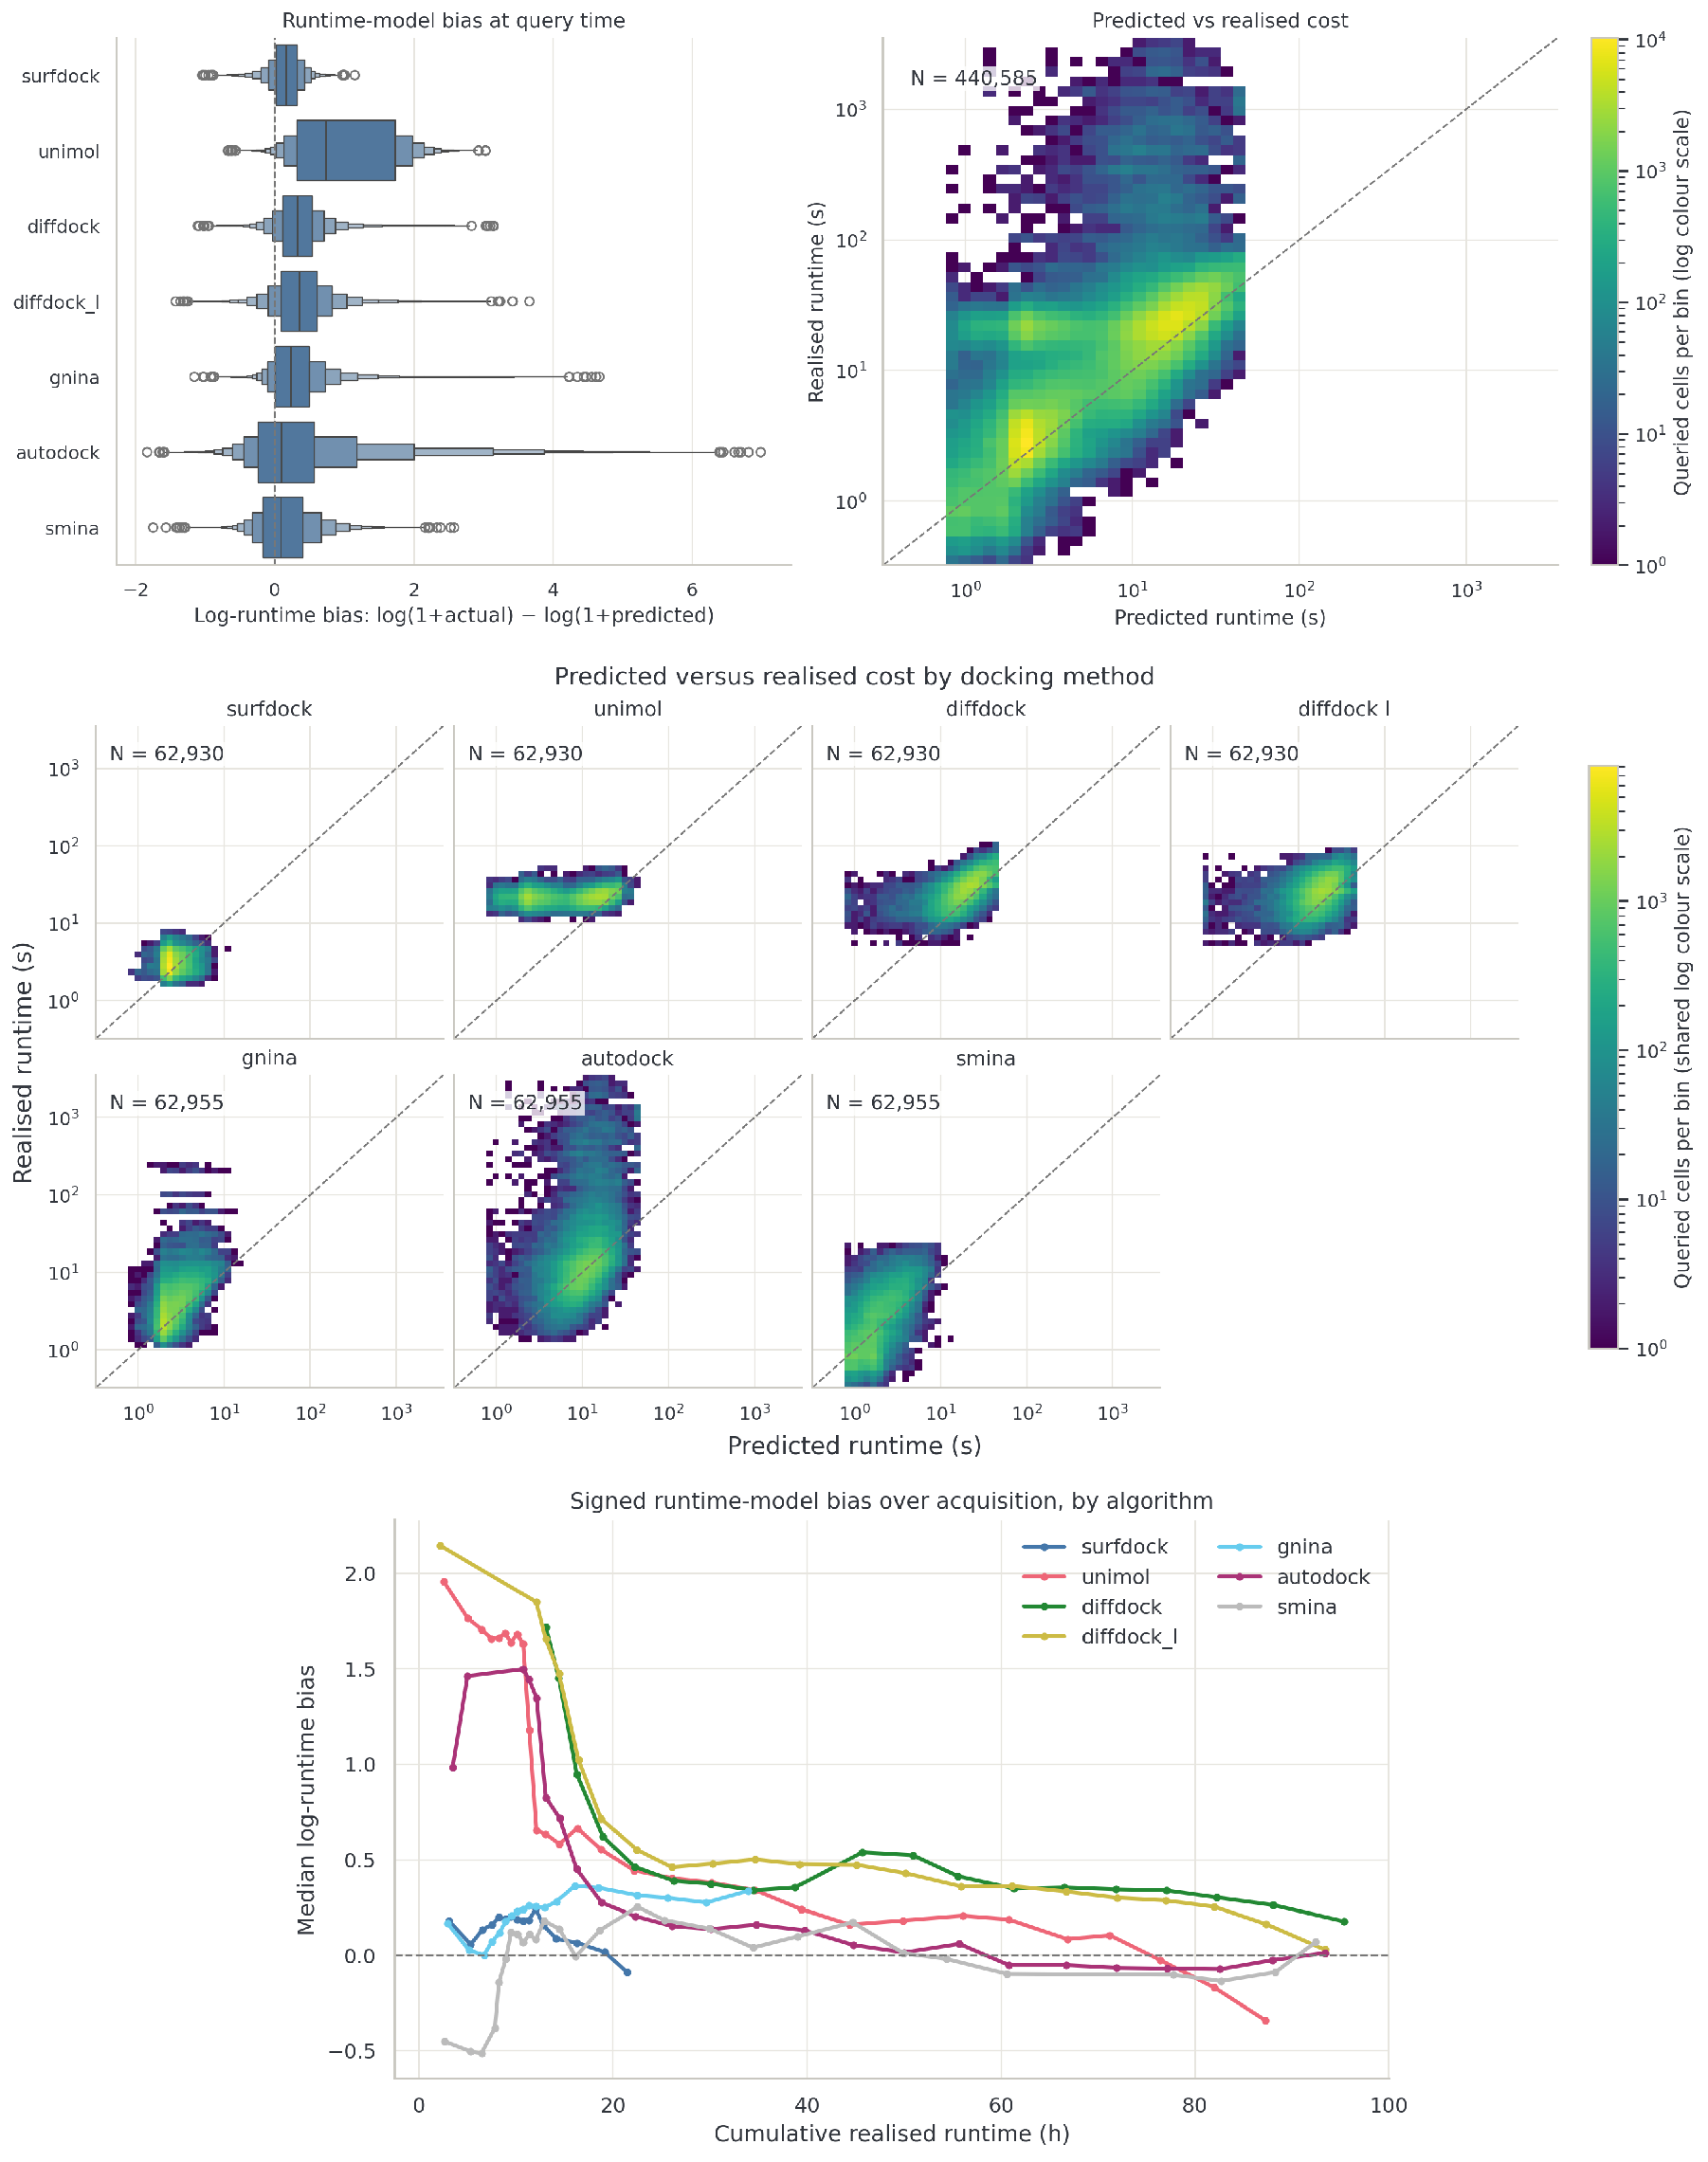
\includegraphics[width=\linewidth]{figures/cost_prediction.pdf}
\caption{Post-warm-start online runtime diagnostics for 440,585 queried-cell records pooled over five cost-aware policies and five folds. Top left: per-algorithm signed log-runtime error; positive values denote underprediction. Top right: pooled density of realized versus predicted runtime. Middle: per-algorithm densities. Bottom: within-bin median signed error over cumulative realized cost. Records can repeat historical cells across policies and overlapping folds.}
\label{fig:cost_prediction}
\end{figure}

For a queried cell, define the signed error $\log(1+C)-\log(1+\widehat C)$, so positive values denote underprediction. In Figure~\ref{fig:cost_prediction}, excluding warm-start observations, the pooled queried-cell distribution is shifted above zero, although errors differ by engine. Uni-Mol and both DiffDock variants are strongly underpredicted initially, whereas Smina is initially overpredicted; several trajectories approach or cross zero later. AutoDock Vina has a less extreme central bias than Uni-Mol but a longer positive tail, corresponding to rare runtimes far beyond its central predictions. The bottom panel pools policies and folds before forming cumulative-cost bins and reports the within-bin median for each engine.

These records describe acquired cells, not calibration over the unqueried pool. The same historical docking outcome can appear in multiple policies and overlapping training folds, so records are not independent docking measurements. The plots document systematic error but neither identify its cause nor evaluate a correction.

\subsection{Effect of cost awareness on acquisition allocation}
\label{app:acquisition-allocation}

\begin{figure}[htbp]
\centering
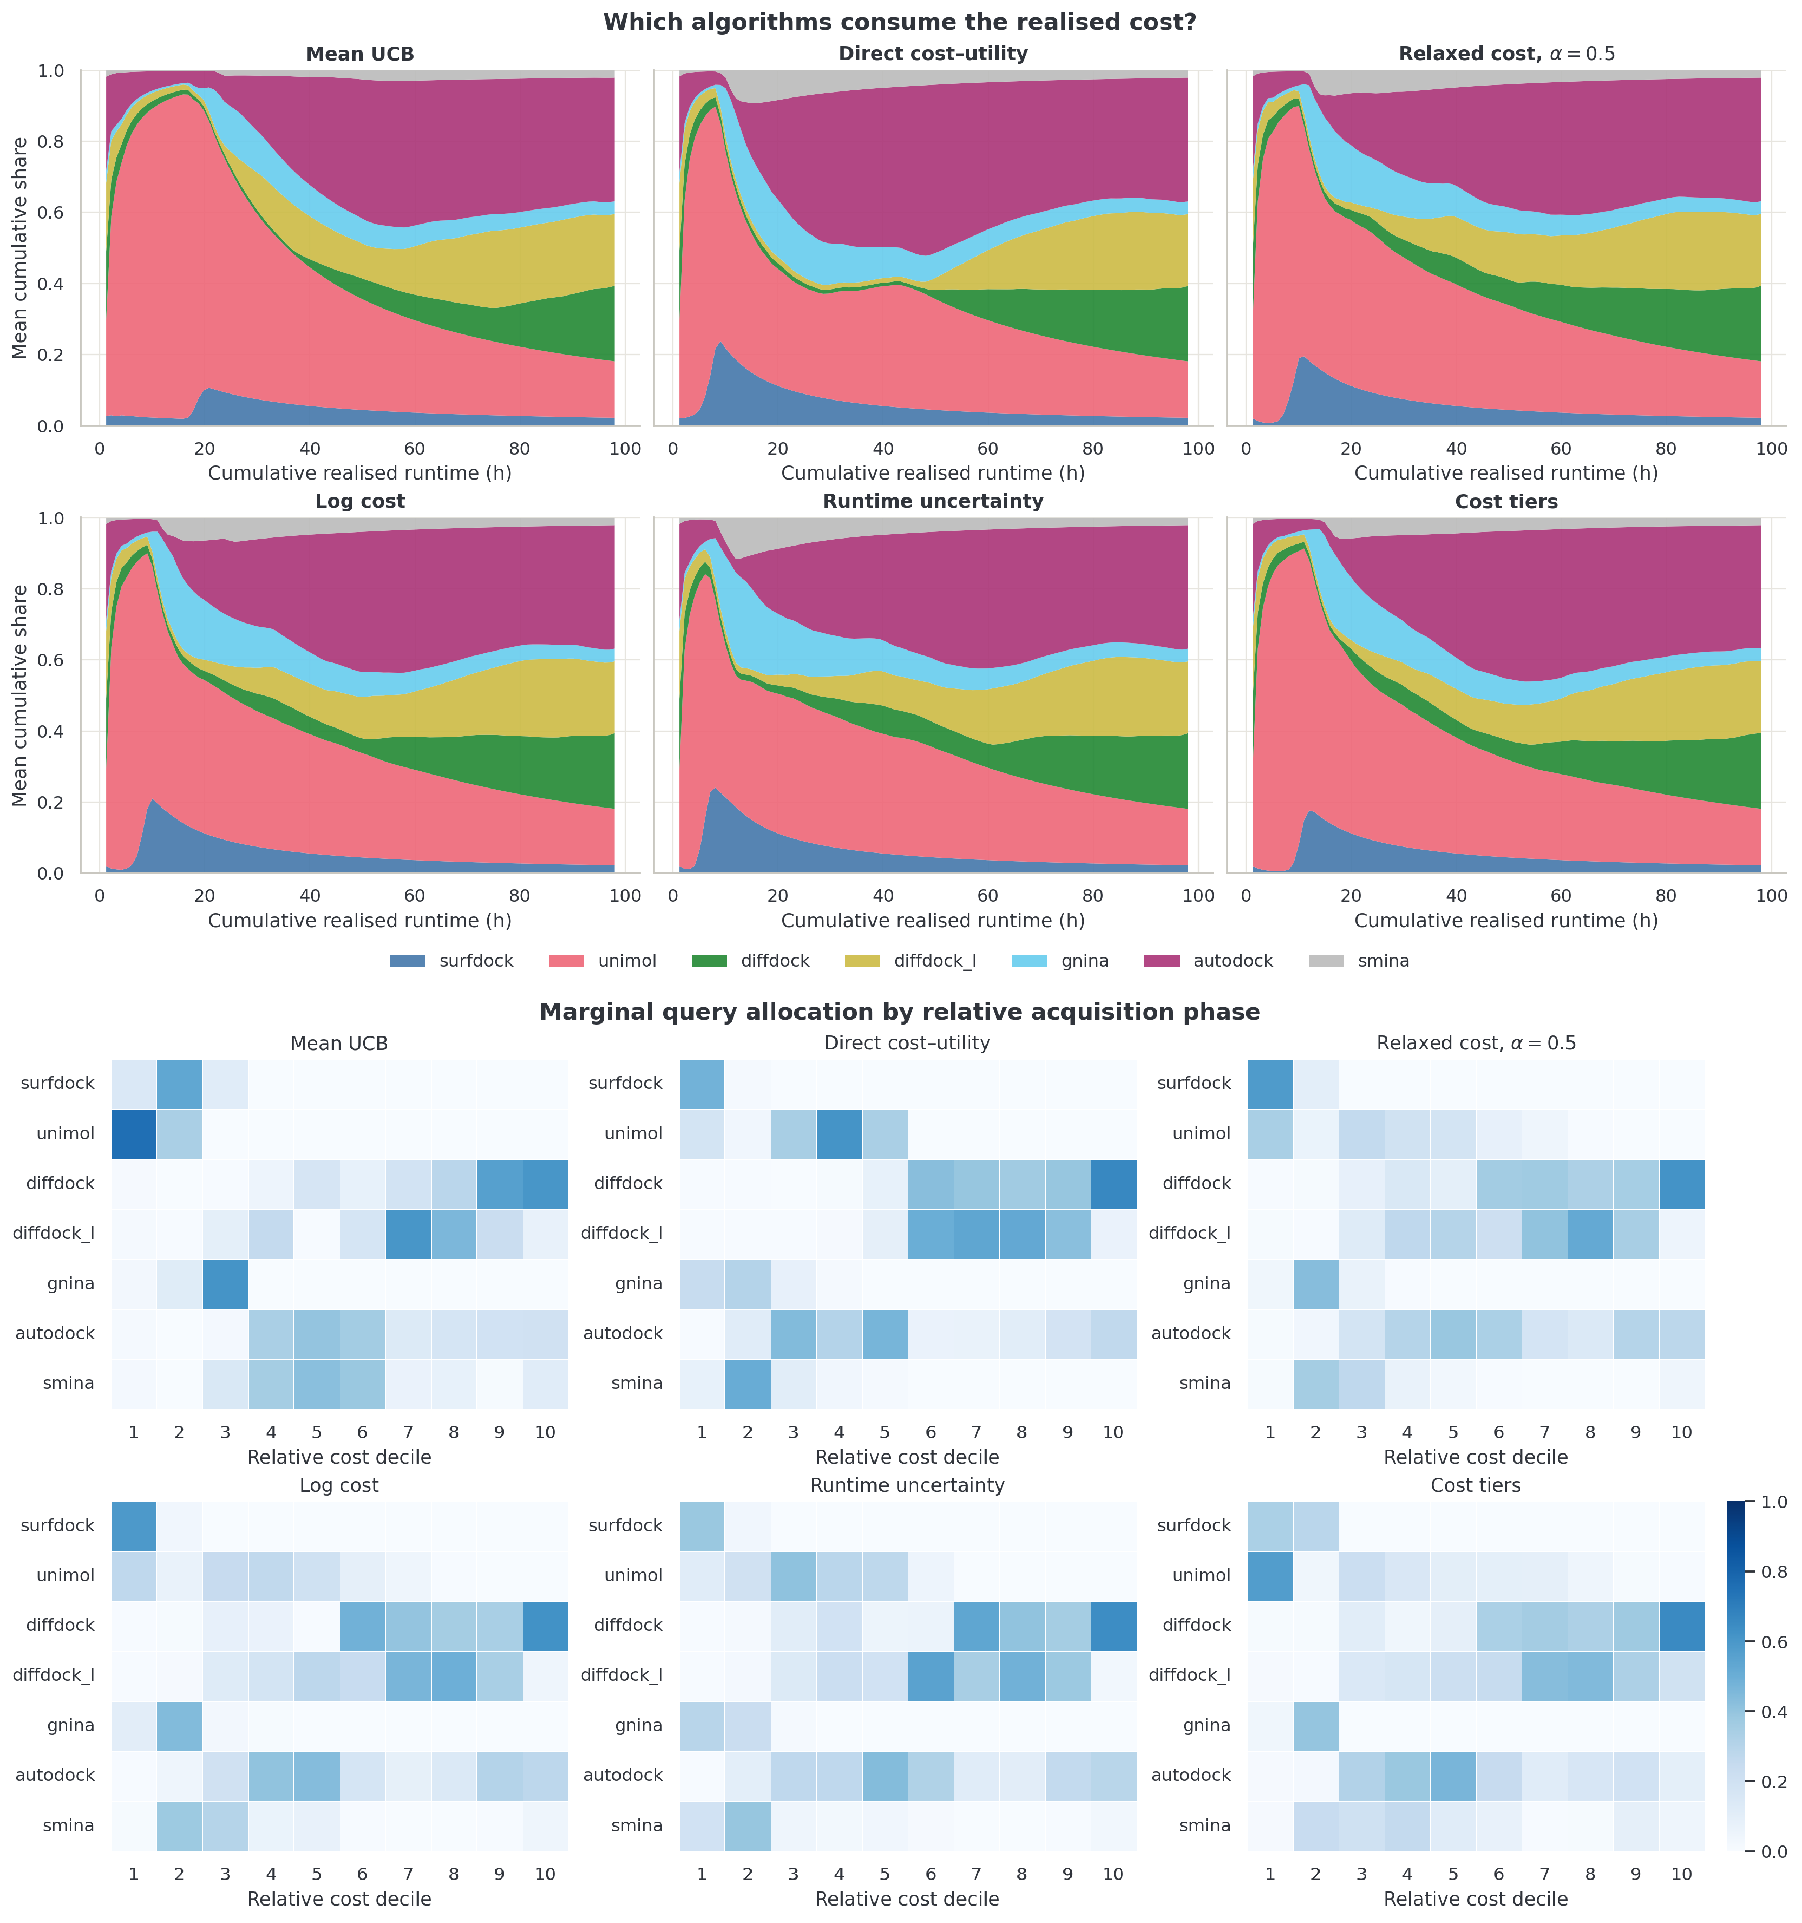
\includegraphics[width=\linewidth]{figures/algorithm_proportion.pdf}
\caption{Top: five-fold mean cumulative realized-cost share by docking engine for each acquisition method. Bottom: fold-mean query share in successive $10\%$ fractions of each fold's full realized training-pool cost.}
\label{fig:algorithm_proportions}
\end{figure}

The common allocation effect is concentrated early (Figure~\ref{fig:algorithm_proportions}). Mean-UCB assigns most first-decile queries to Uni-Mol. The cost-aware variants reduce that concentration to different extents and bring SurfDock, GNINA, and Smina forward. Smina's main query share moves from the middle of the Mean-UCB trajectory to approximately the second or third $10\%$-cost phase. Expensive DiffDock queries are correspondingly deferred. Many cheap Smina queries consume little runtime, while fewer Uni-Mol or extreme AutoDock Vina queries can dominate realized cost. Since every policy eventually observes the same full matrix, these differences describe sequencing.

Signed prediction errors alone do not explain this sequencing. Smina is queried earlier despite early overprediction, whereas Uni-Mol is queried less despite underprediction. This is consistent with coarse between-engine cost separation influencing allocation despite imperfect absolute predictions; it does not show that calibration errors are harmless or establish their causal effect on selector quality.

\begin{figure}[htbp]
\centering
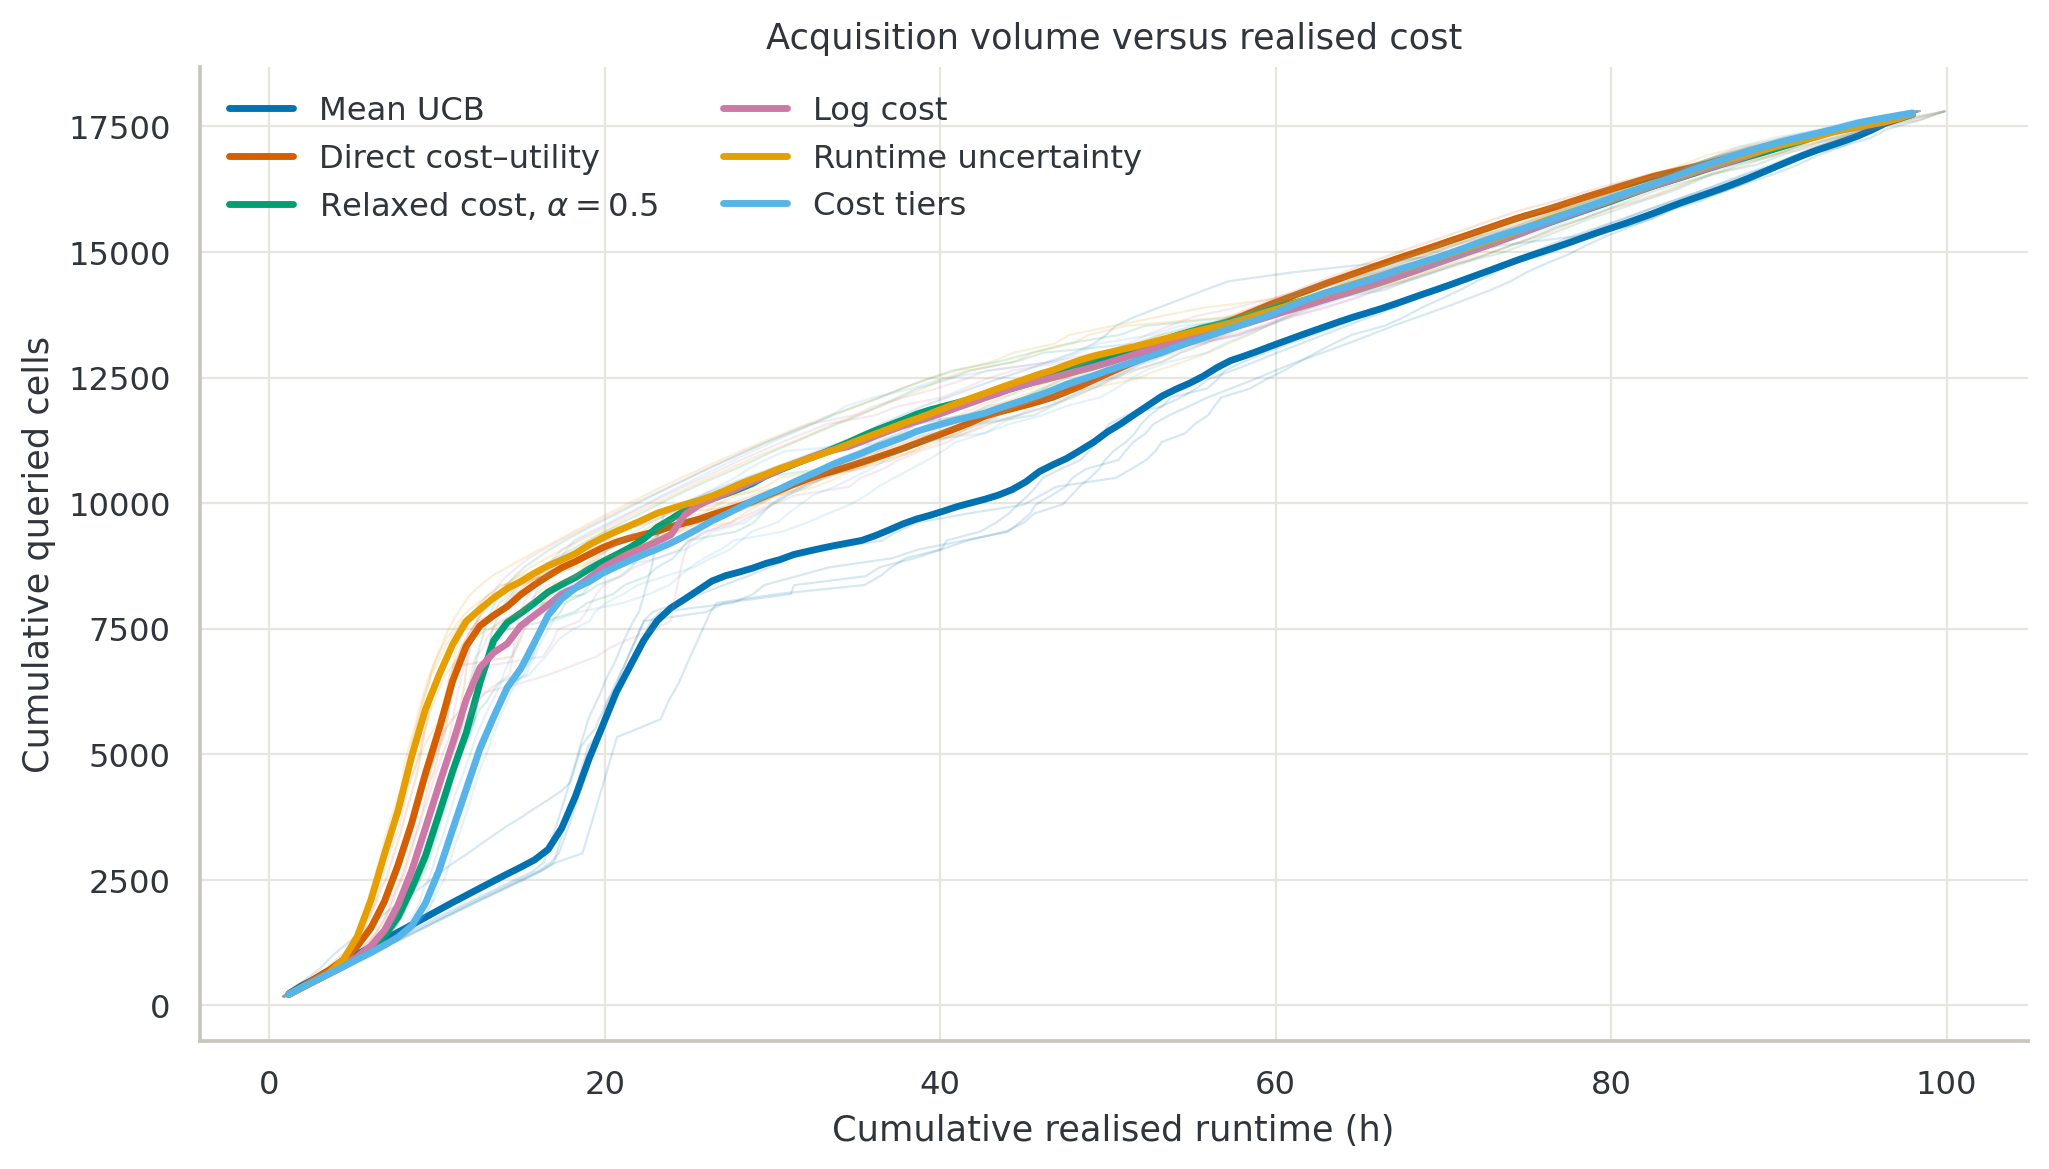
\includegraphics[width=0.75\linewidth]{queried_cells_vs_cost.png}
\caption{Cumulative queried cells versus realized runtime for AL seed~0. Thick curves are five-fold macro means after interpolation over common realized-cost support; faint curves show observed fold trajectories.}
\label{fig:cells2cost}
\end{figure}

Figure~\ref{fig:cells2cost} shows greater acquisition volume for the evaluated cost-aware policies over much of the plotted intermediate-cost range, before convergence when the matrix is exhausted. More acquired cells per realized hour do not by themselves establish greater information value or better downstream decisions.

\begin{figure}[htbp]
\centering
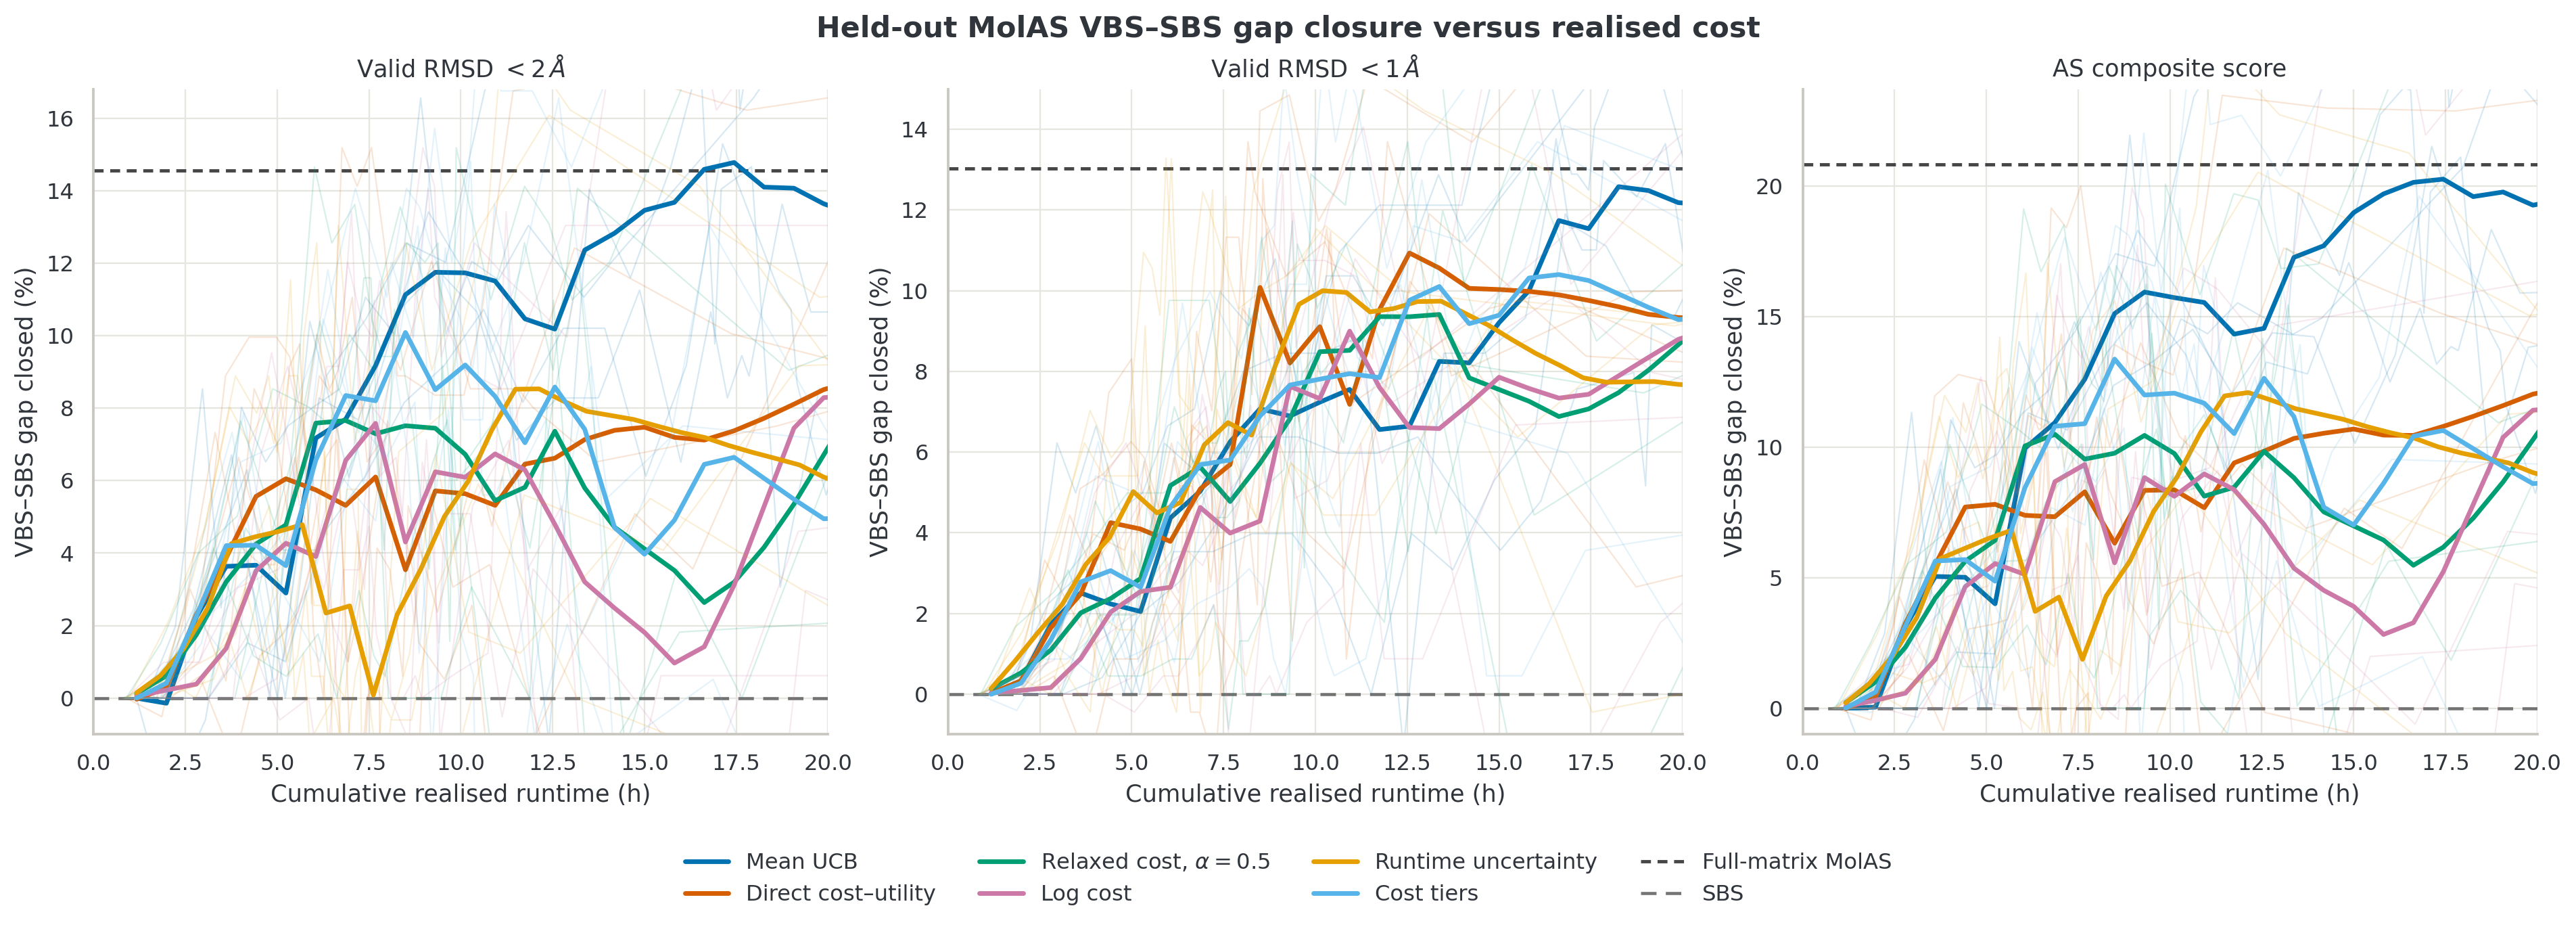
\includegraphics[width=\linewidth]{figures/zoomed_early_downstream_performance_vs_cost.png}
\caption{Held-out SBS--VBS gap closure over the first 20 realized hours. Thick curves are interpolated five-fold macro means; faint curves show fold trajectories. Dashed lines denote SBS ($0\%$ gap closure) and full-matrix MolAS.}
\label{fig:early_downstream}
\end{figure}

Figure~\ref{fig:early_downstream} shows formulation-, endpoint-, and budget-dependent downstream trajectories. Some cost-aware policies exceed the Mean-UCB macro curve over portions of the early-budget range, but these descriptive differences do not establish a statistically significant advantage. Interpolation summarizes evaluated checkpoints; it does not represent a separately trained selector at every plotted runtime. Shared algorithm-level reallocations do not map one-to-one to held-out performance, motivating evaluation of the complete acquisition--completion--selection pipeline.

\subsection{Scope, interpretation, and next steps}
\label{app:next-steps}

Our contribution is an empirical evaluation using established active-learning and matrix-completion methods. The findings concern the evaluated Mean-UCB formulations. Random-cell and pure-uncertainty controls are absent, so improvement over random partial acquisition remains unestablished. Broader comparisons should include joint batch acquisition such as BatchBALD, Pareto-aware policies, and budgeted lookahead. BatchBALD requires joint probabilistic information calculations; SVD disagreement alone is insufficient. The current policies are myopic. These comparisons remain next steps.

MolAS learns from completed targets. An observed-entry-only comparison on identical acquisition histories, using a suitable masked objective, would assess dependence on imputation without treating missing outcomes as failures. Adaptive sampling would still make observed entries selective. Feature-conditioned completion models would test dependence on SVD. Additional acquisition and selector seeds, paired comparisons at prespecified realized-cost checkpoints, and appropriately qualified uncertainty estimates would strengthen statistical characterization. Current fold curves are descriptive, without confidence intervals or formal early-budget significance tests; overlapping training sets and repeated checkpoints are not independent replications. Sensitivity to initialization, $\beta$, SVD ranks, reranking interval, and clipping remains unestablished. These settings define the evaluated configuration rather than validated deployment defaults.

The runtime diagnostics document engine-specific bias on acquired cells, without establishing calibration over the unqueried pool or validating a correction. Calibration using only previously revealed outcomes is a next step, assessed with predictions recorded before each outcome is revealed. Its effects on acquisition and downstream quality require separate evaluation. Guidance on endpoint/budget selection, validation, and monitoring should not be interpreted as an empirically validated stopping or calibration procedure.

Additional datasets, protein--ligand domains, and portfolios would test external validity. Prospective docking is needed to assess hardware transfer, runtime drift, failures, timeouts, retries, and parallel execution. Historical replay does not establish these operational properties, and pose-quality endpoints do not establish experimental hit-discovery benefits. Conclusions remain restricted to the reported retrospective evidence.
